\chapter{Objet}

Ce document a pour but de présenter l'architecture technique de ce projet. Le but de ce projet est de développer un outil de protection et de gestion des licences.

\chapter{Documents de référence}

Documents de spécification :

\begin{itemize}
    \item Spécification Technique des Besoins
    \item Fiches techniques :
	\begin{itemize}
	    \item Injection de code dans un PE
	    \item Génération de licence
	    \item Signature
	    \item Obfuscation de code
	    \item Sécurisation des bases de données
	\end{itemize}
\end{itemize}

\chapter{Terminologie}

\chapter{Configuration requise}

Les éléments matériels nécessaire au développement de cet outil sont :

\begin{itemize}
    \item Un serveur
\end{itemize}

\chapter{Architecture statique}
Afin de réaliser ce projet nous avons choisit de mettre en place l'infrastructure suivante:

\begin{description}
	\item[\textbf{Un serveur web}:]
				C'est ce serveur qui présentera l'interface aux utilisateur et  
				\begin{itemize}
					\item permettra à un client de se créer un compte, demander et 
								télécharger l'outil de generation de licence.
					\item permettra à un administrateur d'accorder et de gérer les licences. 
				\end{itemize}
	\item[\textbf{Un logiciel d'activation}:] 
				sera executé sur la machine de l'utilisateur
				afin de lui permettre de générer une licence. Pour cela il échangera avec
				le serveur des informations sur le matériel physique de la machine, ce 
				qui permettra à ce dernier de générer le fichier de licence.
	\item[\textbf{Outil de Validation}:]
				Outil permettant de vérifier la validité d'une licence, cette outil
				pourra prendre les formes suivantes: 
				\begin{itemize}
				\item Une bibilothèque de fonction qui permettra à un developpeur d'inclure
							dans son code les fonctions de vérification de licence. 
				\item Un programme permettant de greffer directement les fonctions de vérification
							sur un exécutable. 
				\end{itemize}
\end{description}

L'architecture générale de ce projet peut être représenter via 
le schéma n°\ref{fig:fig1}\newline

\begin{figure}[h!]
	\centering
	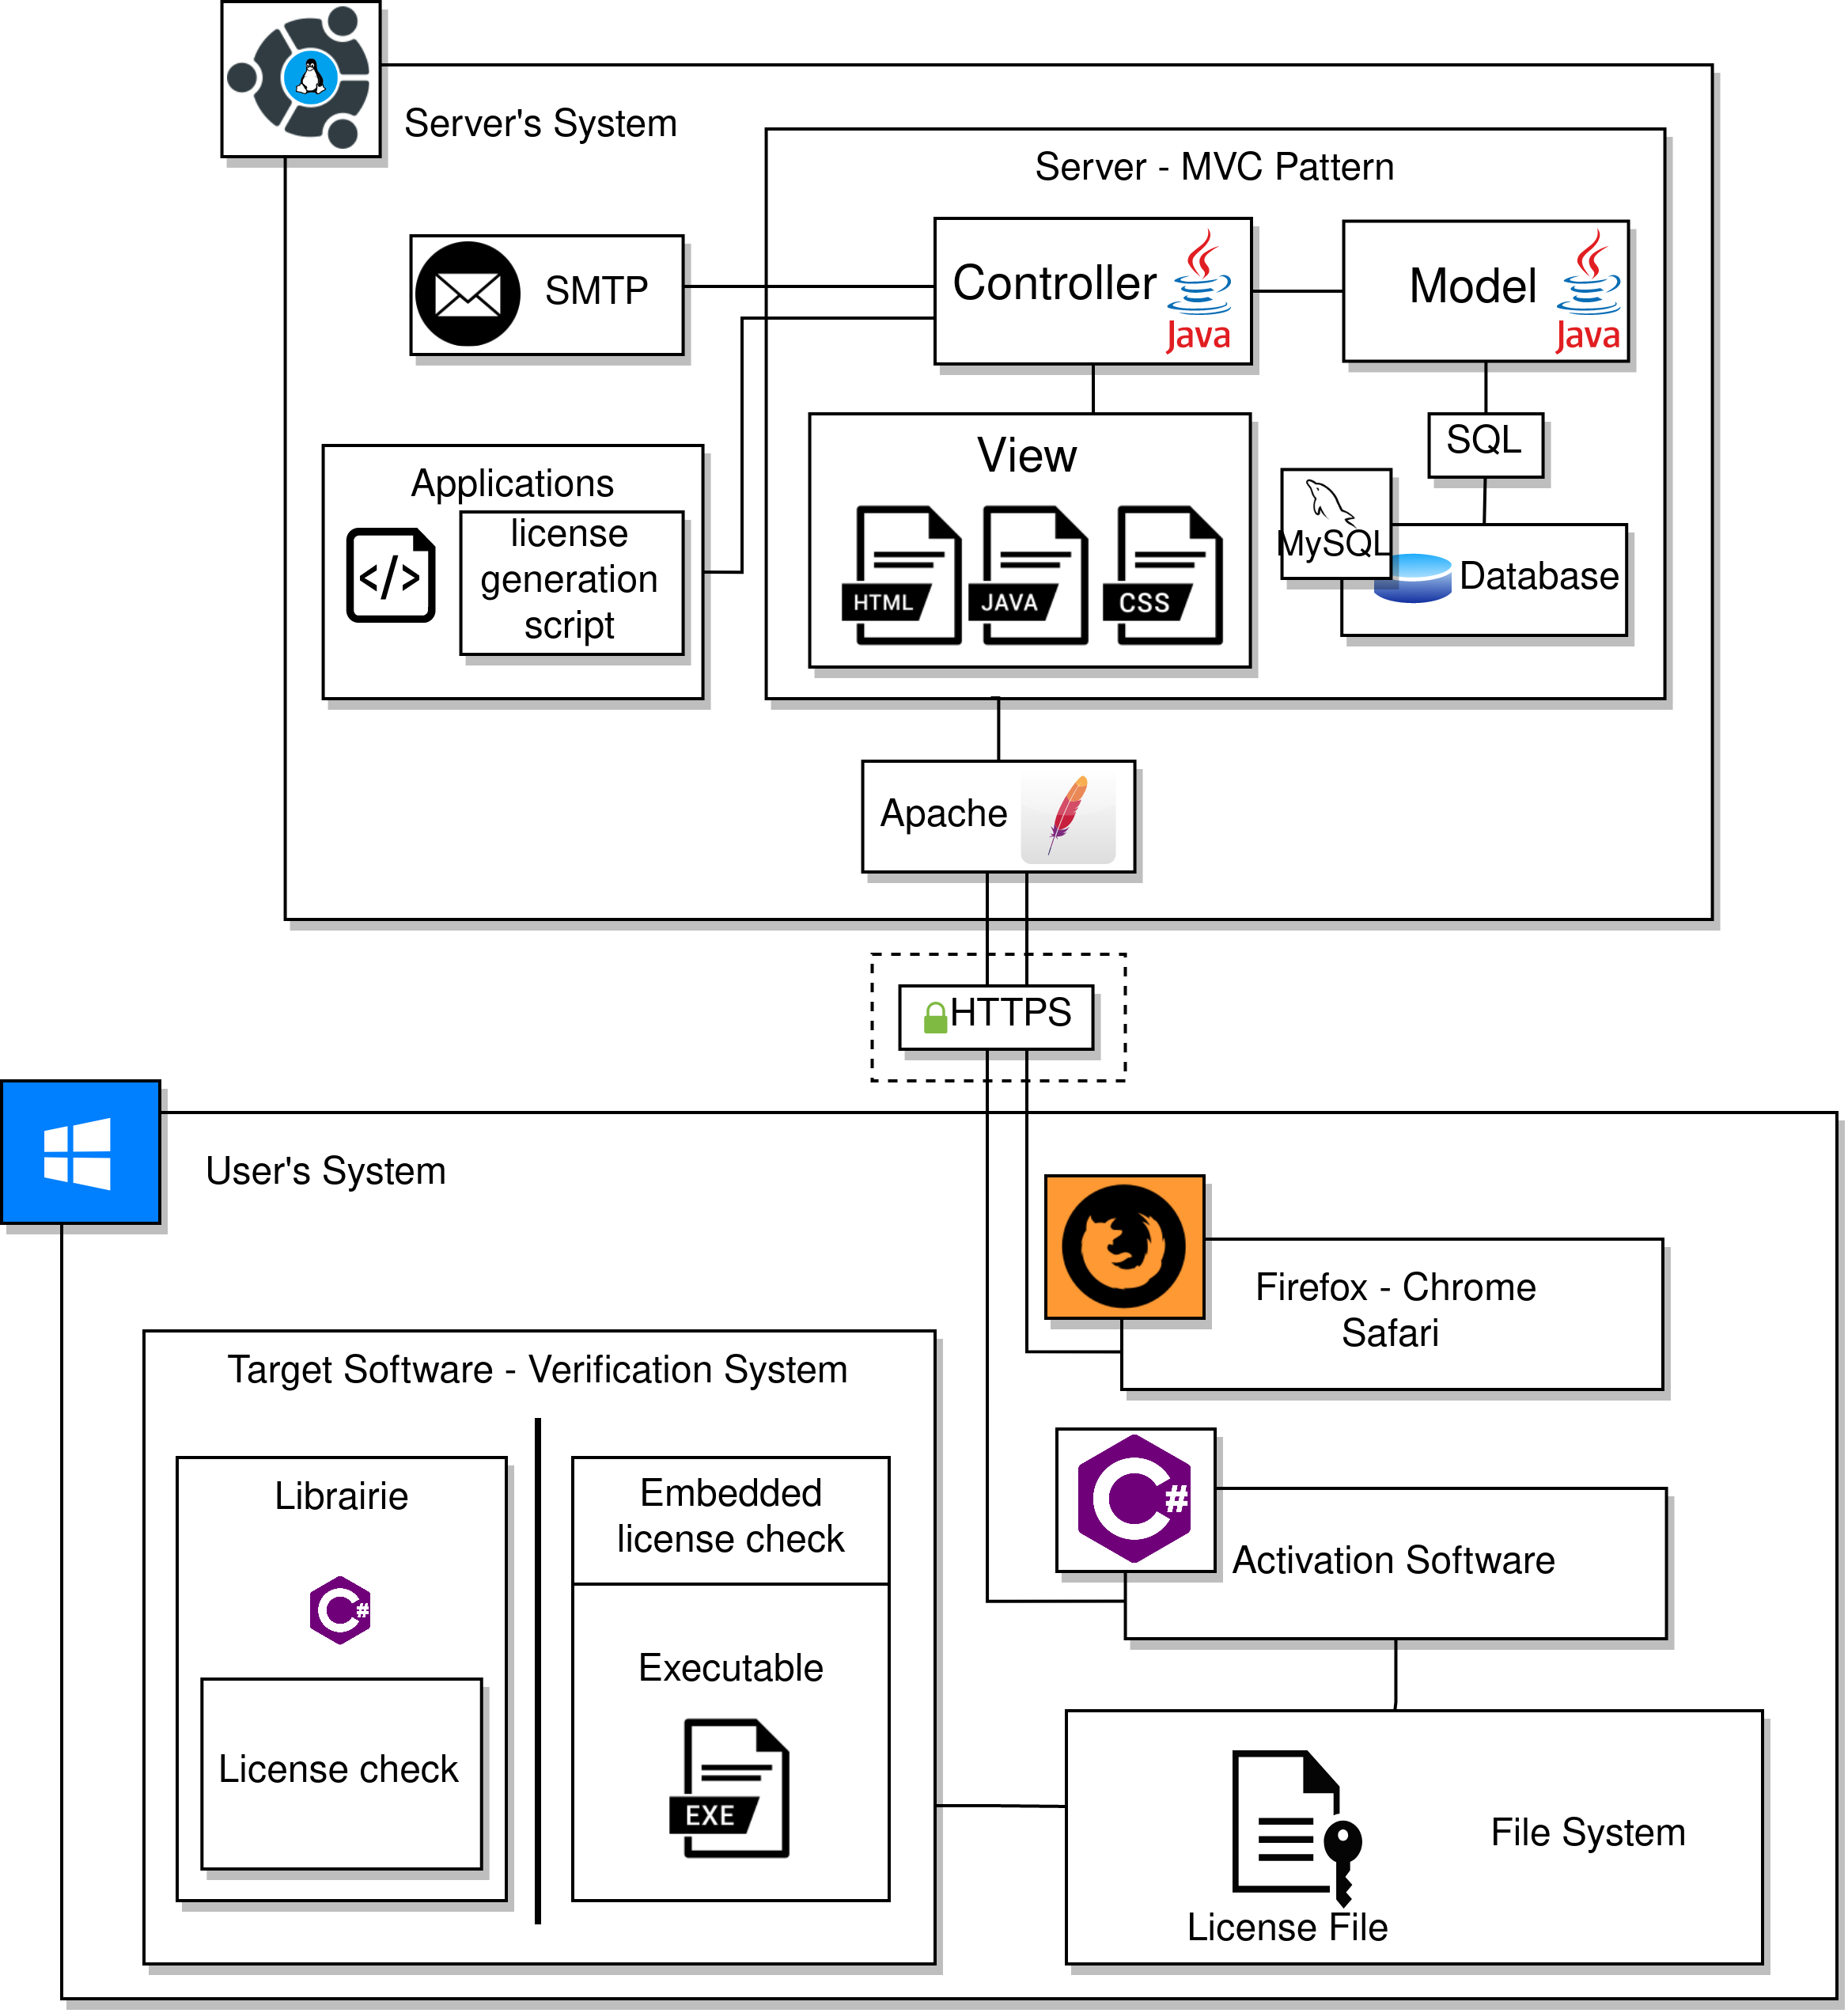
\includegraphics{../png/DAT_general.png}
	\caption{Schéma d'architecture générale}
	\label{fig:fig1}
\end{figure}
\newpage

\section{Constituant `Serveur Applicatif'}

\subsection{Description}

\begin{description}
	\item[\textbf{Rôle}:]
				Le but du serveur est de fournir l'interface principale, programmé 
				en HTML, CSS et JS aux utilisateurs, de stocker dans sa base de donnée
				les informations nécessaires à la génération de licence et enfin de générer 
				les licences.
	\item[\textbf{Propriétés et attributs de caractérisation}:]
	\item[\textbf{Services offerts}:]
				API Rest permettant à au client d'envoyer les informations
				nécéssaires à la génération de la licence (voir \ref{fig:fig2} 				
	\item[\textbf{Dépendances}:]
				Dépend du module de Base de données.
	\item[\textbf{Languages}:]
				HTML, CSS, JS, PHP, SQL, Bash 
	\item[\textbf{Procédé de développement}:]
				Architecture MVC (Model Vue Controler)
	\item[\textbf{Taille et complexité}:]
				Taille importante et complexité élévé.
\end{description}

\subsection{Justifications techniques.}
Utilisation de la pile LAMP (Linux, Apache, MySQL, PHP) car beaucoup de 
support et de documentation (https://www.digitalocean.com/community/tutorials/how-to-install-linux-apache-mysql-php-lamp-stack-ubuntu-18-04)\newline
Possibilité d'automatiser l'installation va un script bash.

\begin{figure}[hp!]
	\caption{API rest}
	\definecolor{getColor}{rgb}{0.28, 0.8, 0.56}
\definecolor{postColor}{rgb}{0.38, 0.68, 0.99}

\usemintedstyle{monokai}
\definecolor{bg}{HTML}{282828} % from https://github.com/kevinsawicki/monokai

\begin{tcolorbox}[title=RestFull API]

	\begin{tcbitemize}[%
    raster columns=7, 
    raster rows=2, 
    raster equal height=rows,
    ]

		% Row I
		\tcbitem[myhbox={}{},
			colback=getColor,colupper=white, 
			fontupper=\sffamily\bfseries\normalsize]	GET
		\tcbitem[raster multicolumn=6, myhbox={}{},
						 fontupper=\ttfamily\bfseries\normalsize] /api/v1/Software/getSoftwareList

		% Row II
		\tcbitem[raster multicolumn=5, myhbox={}{}, 
						 frame hidden, interior hidden] \textbf{Parameters:} 

		\tcbitem[raster multicolumn=2, colback=white, 
						 colupper=black, myhbox={}{}] No parameters 

		% Row III
		\tcbitem[raster multicolumn=3, myhbox={}{}, 
						 frame hidden, interior hidden] \textbf{Response:} 

		\tcbitem[raster multicolumn=2, myhbox={}{}, 
						 frame hidden, interior hidden] \emph{content type}

		\tcbitem[raster multicolumn=2, colback=white, 
						 colupper=black, myhbox={}{}] application/json

		% Row IV
		\tcbitem[raster multicolumn=7, myhbox={}{}]
		\begin{tcbitemize}[raster columns=7, 
											 raster rows=2]
				
			\tcbitem[raster multirow=1, myhbox={}{},
							 fontupper=\sffamily\bfseries\normalsize,
							 frame hidden, interior hidden] 200

			\tcbitem[raster multirow=1, raster multicolumn=6, myhbox={}{}, colback=bg] 
					\begin{minted}[bgcolor=bg, breaklines, breakautoindent=true]{json}
[{
	"SoftwareId" : 0,
	"SoftwareName" : "Logiciel de Gestion de Paye",
	"SoftwareDesc" : "Permet de gérer les payes de vos employés"
}]
				\end{minted}
			
			\tcbitem[raster multirow=1, myhbox={}{},
							 fontupper=\sffamily\bfseries\normalsize,
							 frame hidden, interior hidden] 404

			\tcbitem[raster multirow=1, raster multicolumn=6, myhbox={}{}] Not Found

		\end{tcbitemize}

		% Row V			
		\tcbitem[myhbox={}{},
			colback=postColor,colupper=white, 
			fontupper=\sffamily\bfseries\normalsize]	POST
		\tcbitem[raster multicolumn=6, myhbox={}{},
						 fontupper=\ttfamily\bfseries\normalsize] /api/v1/Licence/requestLicence

	% Row III
	\tcbitem[raster multicolumn=3, myhbox={}{}, 
					 frame hidden, interior hidden] \textbf{Parameters:} 

	\tcbitem[raster multicolumn=2, myhbox={}{}, 
					 frame hidden, interior hidden] \emph{content type}

	\tcbitem[raster multicolumn=2, colback=white, 
					 colupper=black, myhbox={}{}] application/json

	\tcbitem[raster multicolumn=7, myhbox={}{}, colback=bg] 
					\begin{minted}[bgcolor=bg, breaklines, breakautoindent=true]{json}
[{
	"UserMail" : "prenom.nom@mail.com",
	"UserPassword" : "123456seven",
	"SoftwareId" : 0,
	"HardwareHash" : "2e41d4a7-8be7-40ef-8b29-e77aadee37cb"
}]
				\end{minted}
		
	% Row II
	\tcbitem[raster multicolumn=7, myhbox={}{}, 
					 frame hidden, interior hidden] \textbf{Response:} 

	% Row IV
	\tcbitem[raster multicolumn=7, myhbox={}{}]
	\begin{tcbitemize}[raster columns=7, 
										 raster rows=2]
			
		\tcbitem[raster multirow=1, myhbox={}{},
						 fontupper=\sffamily\bfseries\normalsize,
						 frame hidden, interior hidden] 200

		\tcbitem[raster multirow=1, raster multicolumn=6, myhbox={}{}] LicenceFile.key 

		\tcbitem[raster multirow=1, myhbox={}{},
						 fontupper=\sffamily\bfseries\normalsize,
						 frame hidden, interior hidden] 404

		\tcbitem[raster multirow=1, raster multicolumn=6, myhbox={}{}] Not Found

		\end{tcbitemize}

	\end{tcbitemize}
\end{tcolorbox}

	\label{fig:fig2}
\end{figure}
\newpage

\section{Constituant `Base de données'}

\begin{figure}[h!]
	\centering
	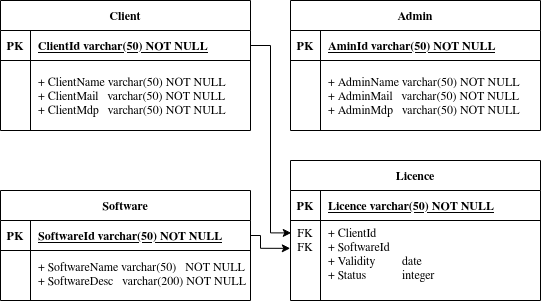
\includegraphics[width=\textwidth]{../png/SQL_table.png}
	\caption{Diagramme UML des Tables de la BDD}
	\label{fig:fig2}
\end{figure}

\subsection{Description}
\begin{description}
	\item[\textbf{Rôle}:]
		Le but de ce module est de permettre de stocker les informations relatives aux
		clients, administrateurs et aux licences. 
	\item[\textbf{Propriétés et attributs de caractérisation}:]
	\item[\textbf{Services offerts}:]
		Fonctions SQL permettant de creer / modifier / supprimer / consulter les 
	  informations relatives aux clients, administrateurs et licences.
	\item[\textbf{Dépendances}:]
		Pas de dépendances.		
	\item[\textbf{Languages}:]
		MySQL.
	\item[\textbf{Procédé de développement}:]
	  Porter une attention partculière à la sécurisation des données, via
	  du chiffrement et à se proteger des attaques du type 'injections SQL'. 
	\item[\textbf{Taille et complexité}:]
		Taille faible et complexité faible. 
\end{description}
\subsection{Justifications techniques.}

\section{Constituant `Logiciel d'Activation'}
\subsection{Description}
\begin{description}
	\item[\textbf{Rôle}:]
		Récuperer les informations matériels sur la machine d'un utilisateur, puis 
		se connecter au serveur afin de générer le fichier de licence.
	\item[\textbf{Propriétés et attributs de caractérisation}:]
	\item[\textbf{Services offerts}:]
	\item[\textbf{Dépendances}:]
		Module Serveur.
	\item[\textbf{Languages}:]
		C\#.
	\item[\textbf{Procédé de développement}:]
		Respect d'une charte de code. 
	\item[\textbf{Taille et complexité}:]
		Taille faible et complexité faible. 
\end{description}

\subsection{Justifications techniques.}

\section{Constituant `Système de véfication - Librairie'}
\subsection{Description}
\begin{description}
	\item[\textbf{Rôle}:]
		Fournir une API pour des programmes en C\# afin de 
		permettre à un developpeur de vérifier une licence dans son code.
	\item[\textbf{Propriétés et attributs de caractérisation}:]

	\newpage

	\item[\textbf{Services offerts}:]
		Listes des fonctions de l'API:
		\begin{minted}{csharp}
/*
 * Récupère l'identifiant de la carte réseau.
 */
public String getNetworkAdapterNo();

/*
 * Récupère le numéro de série du BIOS.
 */
public String getBIOSSerialNo();

/*
 * Récupère le numéro de série du disque.
 */
public String getDiskSerialNo();

/*
 * Récupère les droits d'une licence à partir d'un fichier de
 * licence, renseigné par son chemin.
 */
public String getRights(String pathToLicenseFile);

/*
 * Vérifie la signature à partir des informations du système,
 * de l'identifiant du logiciel, situé dans le programme, et des
 * droits, obtenus à partir du fichier de licence.
 */
public int verifySignature(String pathToLicenseFile);

/*
 * Génère un hashé à partir d'une chaîne de caractères donné
 * en entrée, en utilisant l'algorithme SHA-256.
 */
public String hashWithSHA256(String s);

/*
 * Décode une chaîne de caractères encodée en base64.
 */
public String decodeBase64(String s);
			\end{minted}

			\textbf{Contraintes:}\newline
			Dans un premier temps, les fonctions de l'API pourront être implémentées en utilisant des bibliothèques systèmes
			comme par exemple pour les informations hardware la classe \verb:System.Management:, ou bien la classe
			\verb:System.Security.Cryptography: pour le hash avec SHA-256.\\

			Dans un second temps, nous devrons implanter au maximum les fonctions nous-mêmes et les optimisés dans le but
			de pouvoir intégrer ces fonctions directement dans un exécutable (greffe dans un PE) sans pour autant alourdir
			ou ralentir l'éxécution de l'application.

	\item[\textbf{Dépendances}:]
	\item[\textbf{Languages}:]
		C, C++, C\#
	\item[\textbf{Procédé de développement}:]
		Respect d'un charte de code. 
	\item[\textbf{Taille et complexité}:]
		Taille importante et complexité relative.
\end{description}

\subsection{Justifications techniques.}
Afin de fournir un module le plus indépendant possible afin d'éviter de dépendre d'autres 
librairies externe (et de devoir les monter en mémoire au moment de l'éxécution ce qui 
ralentira le programme) mais aussi dans un but pédagogique nous avons choisit d'implémenter nous même le système cryptographique de signature, le schéma de signature retenu est 
ElGamal \cite{ElGamal}.

\section{Constituant `Système de véfication - Greffe'}
\subsection{Description}
\begin{description}
	\item[\textbf{Rôle}:]
			Outil permettant d'ajouter les fonctions de vérification directement à un
			executable, afin de décharger le developpeur de la necessité de vérifier 
			la licence dans son code.
	\item[\textbf{Propriétés et attributs de caractérisation}:]
	\item[\textbf{Services offerts}:]
	\item[\textbf{Dépendances}:]
	\item[\textbf{Languages}:]
		C, C\#, Python, Bash 
	\item[\textbf{Procédé de développement}:]
		Respect d'un charte de code. 
	\item[\textbf{Taille et complexité}:]
		Taille faible et complexité élevé.
\end{description}

\subsection{Justifications techniques.}

